
\date{\today}
\documentclass[12pt]{article}
\usepackage{graphicx}
\usepackage[T1]{fontenc}


\begin{document}
\section{Przypadki użycia( Use Cases)}
\subsection{Diagram Stanów}
\begin{minipage}[H]{.45\textwidth}
\centering
    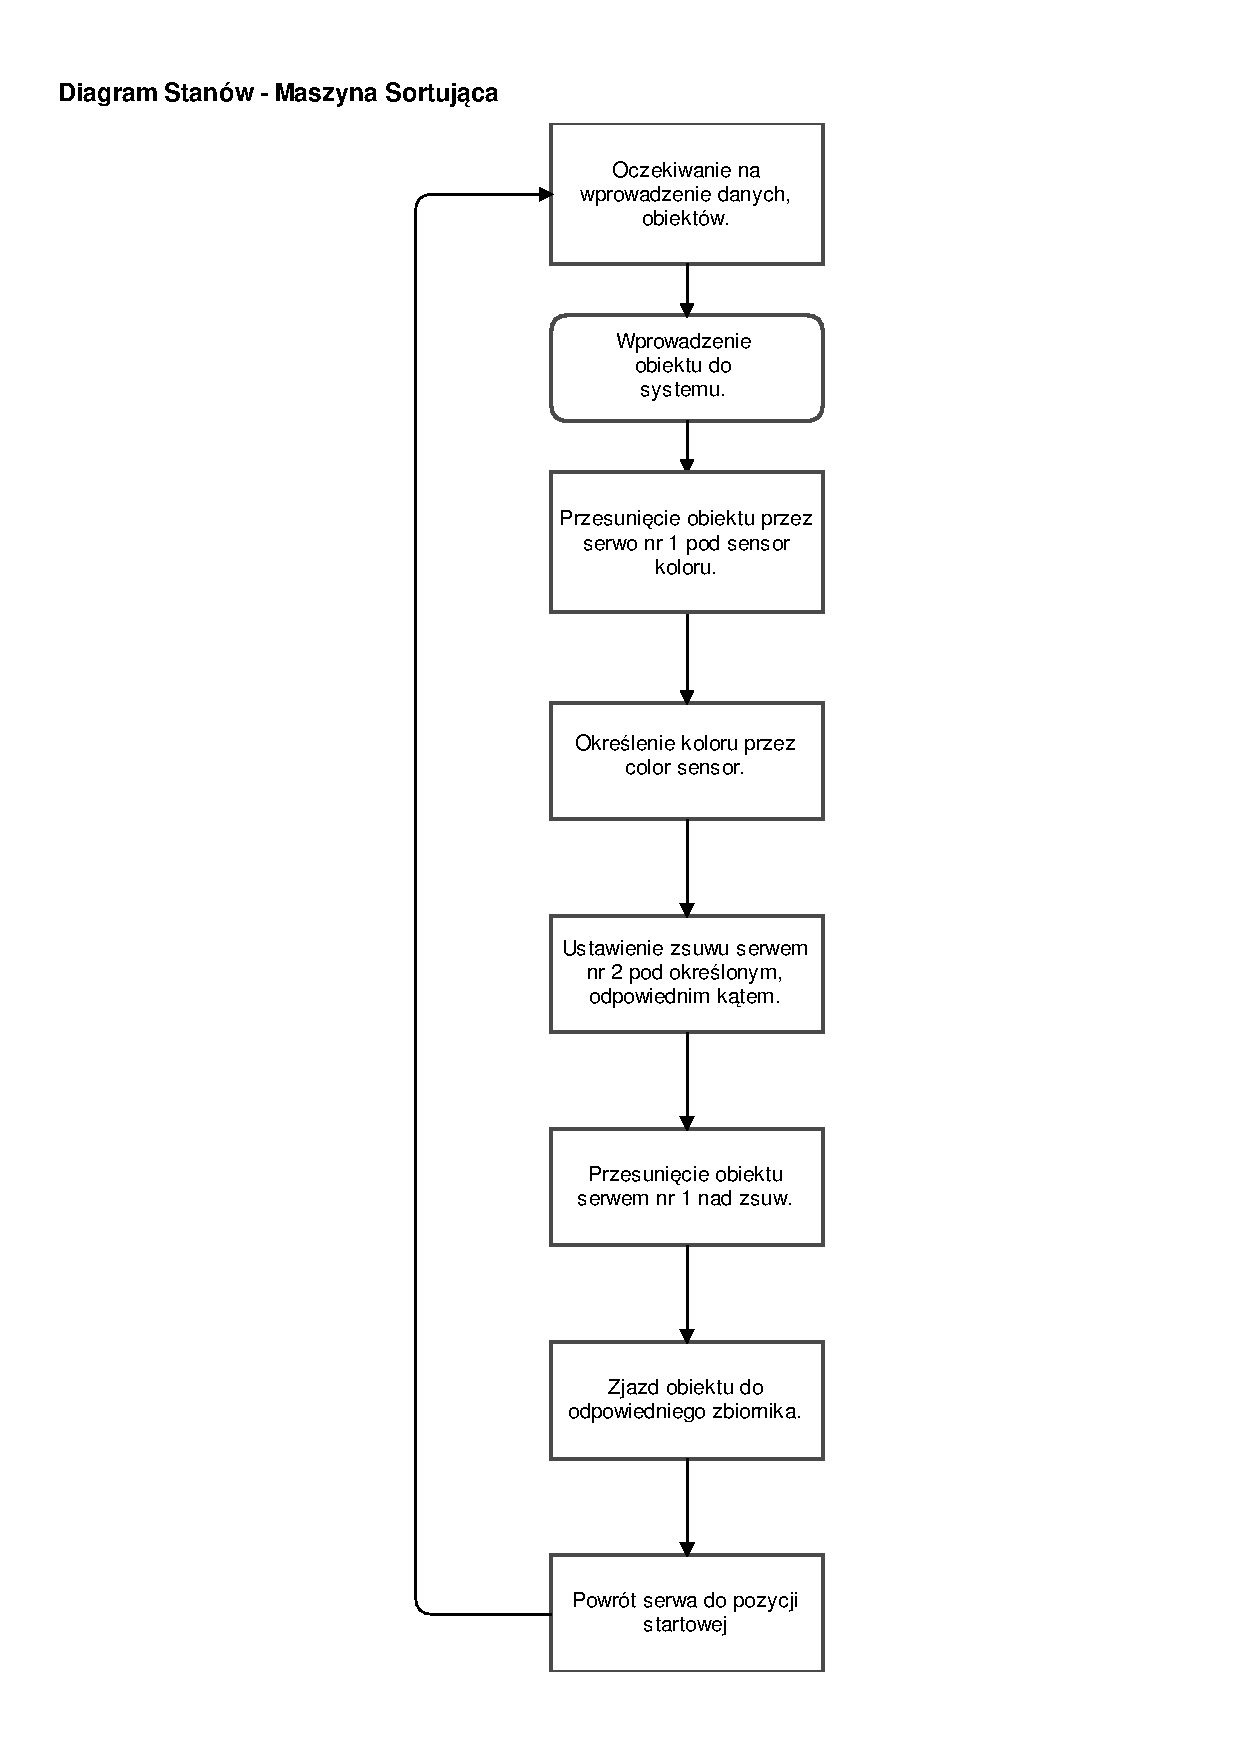
\includegraphics[height=2.8\linewidth]{diagram_stanow.pdf}
\end{minipage}
\subsection{Zasadniczy mechanizm realizowany przez system}
\subsubsection{Uruchomienie Systemu}
\paragraph{Przypadek Użycia:}\mbox{Nr 1}
\paragraph{Priorytet:}\mbox{Wysoki}	
\paragraph{Aktorzy:}\mbox{} \\
Operator uruchamia system, uzyskuje możliwość pracy na urządzeniu.\\
System uzyskuje dostęp do energii( zasilania), dzięki czemu może wykonywać działania.
\paragraph{Opis:}\mbox{} \\
System jest uruchamiany przez operatora dostępnym przyciskiem $ON/OFF$, który daje dostęp do zasilania dla systemu.

\subsubsection{Wprowadzenie Danych}
\paragraph{Przypadek Użycia:}\mbox{Nr 2}
\paragraph{Priorytet:}\mbox{Wysoki}	
\paragraph{Aktorzy:}\mbox{} \\
Operator wprowadza obiekt na wejście.\\
System otrzymuje dane niezbędne do rozpoczęcia działania.
\paragraph{Opis:}\mbox{} \\
Operator wprowadza element na wejście urządzenia. Obiekt Wpada na serwo Nr 1.

\subsubsection{Analiza Obiektu}
\paragraph{Przypadek Użycia:}\mbox{Nr 3}
\paragraph{Priorytet:}\mbox{Wysoki}	
\paragraph{Aktorzy:}\mbox{} \\
System analizuje obiekt podany z wejścia. System otrzymuje informacje o obiekcie na podstawie, których może ustalić kolejne działania.
\paragraph{Opis:}\mbox{} \\
Obiekt znajduję się przy sensorze. Zostaje przebadany pod względem koloru. System zbiera informacje na temat częstotliwości RGB i określa kolor na podstawie zaimplementowanych zasad.

\subsubsection{Ustawienie Zsuwu}
\paragraph{Przypadek Użycia:}\mbox{Nr 4}
\paragraph{Priorytet:}\mbox{Wysoki}	
\paragraph{Aktorzy:}\mbox{} \\
System na podstawie posiadanych informacji ustawa zsuw w odpowiednim kącie.
\paragraph{Opis:}\mbox{} \\
System na podstawie zebranych informacji ustawia zsuw wykorzystując serwo nr 2. Pochylnia ustawiona jest pod takim kątem, aby wpaść do odpowiedniego kontenera.

\subsubsection{Zwolnienie obiektu}
\paragraph{Przypadek Użycia:}\mbox{Nr 5}
\paragraph{Priorytet:}\mbox{Wysoki}	
\paragraph{Aktorzy:}\mbox{} \\
System przenosi obiekt do zsuwu. 
Operator uzyskuje uporządkowany obiekt w oczekiwanym miejscu.
\paragraph{Opis:}\mbox{} \\
System przekazuje przez serwo nr 1 obiekt nad poprawnie ustawiony zsuw, przez  co zwalnia obiekt,a ten toczy się do odpowiedniego kontenera. Po czym serwo nr 1 wraca do początkowej pozycji, a system oczekuje na kolejny obiekt.

\subsection{Inne Przypadki Użycia}
\paragraph{Aktorzy:}\mbox{} \\
Użytkownik resetuje serwa do pozycji $zerowej$.
\paragraph{Opis:}\mbox{} \\
Użytkownik resetuje serwa do pozycji $zerowej$ przyciskiem reset z panelu.

\subsection{Ekstremalne Przypadki Użycia}
\paragraph{Priorytet:}\mbox{Niski}	
\paragraph{Aktorzy:}\mbox{} \\
Użytkownik dodaje nowy kontener.
\paragraph{Opis:}\mbox{} \\
Zostaje dodana specyfikacja częstotliowści i nowy kąt pod jakim ma ustawić się zsuw po rozpoznaniu.






\end{document}